\documentclass[aspectratio=169]{beamer}

\usepackage{global-macros}
\usepackage{graphicx}
\graphicspath{{../fig}}
\usepackage{algpseudocode, algorithm}
\usepackage{biblatex}

\vfuzz=30pt


\addbibresource{../bib/bibliography.bib}

\title{NPIV estimation through functional SGD}
\author{Student: Caio Lins
        \\ Advisor: Yuri Saporito
}
\institute{EMAp -- FGV}
\date{\today}

\titlegraphic{
    
\includegraphics[width=3cm]{logo.png}
}

\AtBeginSection[]
{%
  \begin{frame}
    \frametitle{Summary}
    \tableofcontents[currentsection]
  \end{frame}
}

\addtobeamertemplate{navigation symbols}{}{%
    \usebeamerfont{footline}%
    \usebeamercolor[fg]{footline}%
    \hspace{1em}%
    \insertframenumber/\inserttotalframenumber
}

\newcommand{\boldf}{\boldsymbol{f}}

\newcommand{\hstar}{h^{ \star }}
\newcommand{\risk}{\mathcal{R}}
\newcommand{\loss}{\ell}
\renewcommand{\hat}{\widehat}
\newcommand{\iid}{\overset{\mathrm{iid}}{\sim}}
\DeclareMathOperator{\diam}{diam}
\newcommand{\data}{\mathcal{D}}
\newcommand{\dataproj}{\mathcal{D}_{ \mathrm{proj} }}


\begin{document}

    \frame{\titlepage}

    \section{Instrumental Variable Regression}

    \begin{frame}{Instrumental Variables}
        \begin{itemize}
            \item<1-> Regression: $ Y = \hstar ( X ) + \varepsilon $, with $ \mean [ \varepsilon ] = 0 $.
                Find $ \hstar $.
            \item<2-> Minimizing $ \mse ( h ) = \mean [ ( Y - h ( X ) )^2 ] $ gives 
                \begin{equation*}
                    \hat{ h } ( X ) = \mean [ Y \mid X ] = \hstar ( X ) + \mean [ \varepsilon \mid X ]
                .\end{equation*}
            \item<3-> What if $ \mean [ \varepsilon \mid X ] \neq 0 $?
                That is, if $ X $ is \emph{endogenous}?
        \end{itemize}
    \end{frame}

    \begin{frame}{Instrumental Variables}
        \begin{itemize}
            \item<1-> Suppose we have access to a variable $ Z $ such that
                \begin{enumerate}
                    \item<2-> $ Z $ influences $ X $, that is, $ Z \notindep X $;
                    \item<3-> $ Z $ is \emph{exogenous}, that is, $ \mean [ \varepsilon \mid Z ] = 0 $.
                \end{enumerate}
                \uncover<4->{$ Z $ is called an \emph{instrumental variable}.}
        \end{itemize}
    \end{frame}

    \begin{frame}{Instrumental Variables}
        \begin{figure}[t]
            \begin{center}
                \begin{tikzpicture}[node distance=3cm]
                    \node[circle,draw] at (0,0) (X) {$X$};
                    \node[circle,draw,right of=X] (Y) {$Y$};
                    \node[circle,draw,left of=X] (Z) {$Z$};
                    \node[circle,draw,above of=X,xshift=1.5cm,yshift=-1.5cm] (eps) {$\varepsilon$};
                    \draw[->] (X) -- (Y);
                    \draw[->] (Z) -- (X);
                    \draw[->] (eps) -- (X);
                    \draw[->] (eps) -- (Y);
                \end{tikzpicture}
            \end{center}
            \caption{Causal diagram representing an instrumental variable for an endogenous covariate.}
        \end{figure}
    \end{frame}

    \begin{frame}{Instrumental Variables}
        Example:
        \begin{itemize}
            \item $ X = $ is smoker?
            \item $ Y = $ general health.
            \item $ Z = $ tax rate on tobacco products.
            \item $ \varepsilon = $ depression, self care.
        \end{itemize}
        \begin{figure}[t]
            \begin{center}
                \begin{tikzpicture}[node distance=3cm]
                    \node[circle,draw] at (0,0) (X) {$X$};
                    \node[circle,draw,right of=X] (Y) {$Y$};
                    \node[circle,draw,left of=X] (Z) {$Z$};
                    \node[circle,draw,above of=X,xshift=1.5cm,yshift=-1.5cm] (eps) {$\varepsilon$};
                    \draw[->] (X) -- (Y);
                    \draw[->] (Z) -- (X);
                    \draw[->] (eps) -- (X);
                    \draw[->] (eps) -- (Y);
                \end{tikzpicture}
            \end{center}
        \end{figure}
    \end{frame}

    \begin{frame}{Linear Model}
        \begin{equation*}
            \bY = \bX \bstar + \varepsilon
        .\end{equation*}
        \begin{itemize}
            \item<2-> $ \betaols = ( \bX^{ \trp } \bX )^{ -1 } \bX^{ \trp } \bY $ is biased and inconsistent;
            \item<3-> $ \betaiv = ( \hat{ \bX }^{ \trp } \hat{ \bX } )^{ -1 } \hat{ \bX }^{ \trp } \bY $, where
                \begin{equation*}
                    \hat{ \bX } = \bZ ( \bZ^{ \trp } \bZ )^{ -1 } \bZ^{ \trp } \bX
                ,\end{equation*}
                is unbiased and consistent.
            \item<3-> Two Stages Least Squares (2SLS).
        \end{itemize}
    \end{frame}

    \begin{frame}{Linear Model}
        \begin{figure}[htb]
            \begin{center}
                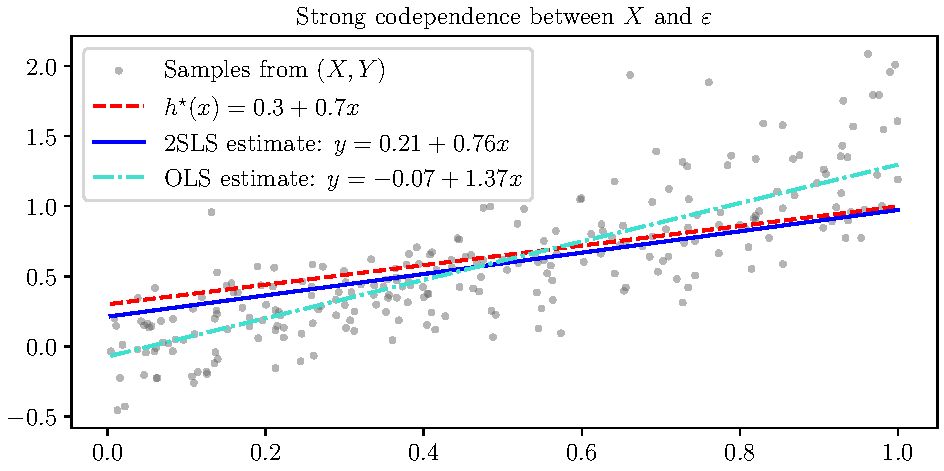
\includegraphics[width=.9\textwidth]{tsls_examples.pdf}
            \end{center}
        \end{figure}
    \end{frame}

    \section{Nonparametric Instrumental Variable Regression}

    \begin{frame}{Problem formulation}
        \begin{equation*}
            Y = \hstar ( X ) + \varepsilon, \quad \text{with $ \mean [ \varepsilon \mid X ] \neq 0 $, $ Z \notindep X $ and $ \mean [ \varepsilon \mid Z ] = 0 $}
        .\end{equation*}
        \begin{itemize}
            \item<1-> We have access to $ \left\{ ( X_{ i }, Y_{ i }, Z_{ i } ) \right\} $;
            \item<2-> We assume $ \hstar \in L^2 ( X ) = \left\{ h : \mean [ h ( X )^2 ] < \infty \right\} $.
            \item<3-> Conditioning in $ Z $:
                \begin{equation*}
                    \mean [ Y \mid Z ] = \mean [ \hstar ( X ) \mid Z ] \iff
                    {\color{blue} r = \meanop [ \hstar ]}
                ,\end{equation*}
                where $ r ( Z ) = \mean [ Y \mid Z ] $ and $ \meanop : L^2 ( X ) \to L^2 ( Z ) $ is the \emph{conditional expectation operator}:
                \begin{equation*}
                    \meanop [ h ] ( z ) = \mean [ h ( X ) \mid Z = z \ ]
                .\end{equation*}
            \item<4-> $\mathrm{I}$ll posed problem.
        \end{itemize}
    \end{frame}

    \begin{frame}{Classical Approaches}
        \let\tempone\itemize
        \let\temptwo\enditemize
        \renewenvironment{itemize}{\tempone\addtolength{\itemsep}{0.7\baselineskip}}{\temptwo}
        Problem: $ r = \meanop [ \hstar ] $, where $ r ( Z ) = \mean [ Y \mid Z ] $ and $ \meanop [ h ] ( Z ) = \mean [ h ( X ) \mid Z ] $.

        \begin{itemize}
            \item<2-> Nonlinear Two Stages Least Squares \cite{newey2003}:
                \begin{itemize}
                    \item $ \hstar ( x ) \approx \sum_{ j=1 }^{ J } \gamma_{ j } p_{ j } ( x ) $;
                    \item $ \mean [ p_{ j } ( X ) \mid Z = z \ ] \approx \sum_{ i=1 }^{ n } a_{ ji } q_{ i } ( z ) $.
                \end{itemize}

            \item<3-> Iterated Tikhonov regularization \cite{darolles2011}:
                \begin{itemize}
                    \item $ \argmin_{ h } \ \norm{ \meanop [ h ] - r }_{ L^2 ( Z ) }^2 + \alpha \norm{ h }_{ L^2 ( X ) }^2 = ( \meanop^{ * } \meanop + \alpha I )^{ -1 } \meanop^{ * } [ r ] $;
                    \item $ h_{ k+1 } = ( \meanop^{ * } \meanop + \alpha I )^{ -1 } [ \meanop^{ * } r + h_{ k } ] $
                \end{itemize}
        \end{itemize}
    \end{frame}

    \section{Stochastic Approximate Gradient Descent IV}

    \begin{frame}{Risk measure}
        We know that $ \hstar $ satisfies
        \begin{equation*}
            r = \meanop [ \hstar ]
        .\end{equation*}
        \begin{itemize}
            \item<2-> Define the risk
                \begin{equation*}
                    \risk ( h ) = \mean [ \ell ( r ( Z ), \meanop [ h ] ( Z ) ) ]
                .\end{equation*}
                E.g., if $ \ell ( y, y' ) = ( y - y' )^2 $:
                \begin{align*}
                    \risk ( h )
                    &= \mean \left[
                        \left(
                            r ( Z ) - \meanop [ h ] ( Z )
                        \right)^2
                    \right] \\
                    &= \mean \left[
                        \left(
                            \meanop [ h - \hstar ] ( Z )
                        \right)^2
                    \right]
                .\end{align*}
        \end{itemize}
    \end{frame}

    \begin{frame}{Gradient Descent}
        \begin{equation*}
            \risk ( h ) = \mean [ \ell ( r ( Z ), \meanop [ h ] ( Z ) ) ]
        .\end{equation*}
        \begin{itemize}
            \item<2-> We showed that
                \begin{align*}
                    \nabla \risk ( h ) ( x )
                    &= \meanop^{ * } [ \partial_{ 2 } ( r ( Z ), \meanop [ h ] ( Z ) ) ] \\
                    &= \mean [ {\color{blue} \Phi ( x, Z ) \partial_{ 2 } ( r ( Z ), \meanop [ h ] ( Z ) )} ]
                ,\end{align*}
                where $ \Phi ( x, z ) = \frac{ p_{ XZ } ( x, z ) }{ p_{ X } ( x ) p_{ Z } ( z ) } $.
            \item<3-> The term in blue is a stochastic gradient.
            \item<4-> Problem: do not know $ \Phi, \meanop $ nor $ r $.
                Only have access to $ \left\{ ( X_{ i }, Y_{ i }, Z_{ i } ) \right\} $.
        \end{itemize}
    \end{frame}

    \begin{frame}{Projected Gradient Descent}
        \begin{itemize}
            \item<1-> Our regularization: look for solutions in $ \mathcal{H} \subseteq L^2 ( X ) $;
            \item<2-> $ \mathcal{H} $ is convex, closed and bounded.
            \item<3-> E.g. for $ A > 0 $:
        \begin{equation*}
            \mathcal{H} = \left\{ h \in L^2 ( X ) : \abs{ h ( x ) } \leq A \ \forall x \right\}
        .\end{equation*}
        \end{itemize}
    \end{frame}

    \begin{frame}{Stochastic Approximate Gradient Descent}
        \begin{itemize}
            \item<1-> $ \nabla \risk ( h )(x) = \mean [ {\color{blue}\Phi ( x, Z ) \partial_{ 2 } ( r ( X ), \meanop [ h ] ( Z ) )} ] $, but we do not know $ \Phi, r, \meanop $;
            \item<2->  Assume we have estimators $ \hat{ \Phi }, \hat{ r } $ and $ \hat{ \meanop } $, so that
                \begin{equation*}
                    u_{ h } ( x ) = {\color{blue}\hat{ \Phi } ( x, Z ) \partial_{ 2 } ( \hat{ r } ( Z ), \hat{ \meanop } [ h ] ( Z ) )}
                \end{equation*}
                is an \emph{approximate stochastic gradient} for $ \risk $ at $ h $.
        \end{itemize}
    \end{frame}

    \begin{frame}{Kernel Methods}
        \begin{itemize}
            \item<1-> Kernel Ridge Regression to compute $ \hat{ \Phi }, \hat{ r } $ and $ \hat{ \meanop } $;
            \item<2-> Reproducing Kernel Hilbert Space (RKHS) as a class of approximating functions $\implies$ closed form solutions;
            \item<3-> $ \hat{ \meanop } $ is tricky.
                We used KIV's first stage \cite{singh2019}.
        \end{itemize}
    \end{frame}

    \begin{frame}{SAGD--IV}
        \begin{algorithm}[H]\label{algo: sagdiv}
            \caption{SAGD--IV}
            \SetKwInOut{Input}{input}
            \SetKwInOut{Output}{output}
            \Input{
                Samples $ \left\{ ( \bz_{ m } )_{ m=1 }^{ M } \right\} $.
                Estimators $ \hat{ \Phi }, \hat{ r } $ and $ \hat{ \meanop } $.
                Sequence of learning rates $ ( \alpha_{ m } )_{ m=1 }^{ M } $.
            }
            \Output{ $ \hat{ h } $ }
            \For{$ 1 \leq m \leq M $}{
            Set $ u_{ m } = {\color{blue}\hat{ \Phi } ( \cdot , \bz_{ m } ) \partial_{ 2 } \ell \left( \hat{ r } ( \bz_{ m } ), \hat{ \meanop } [ \hat{ h }_{ m - 1 } ] ( \bz_{ m } ) \right)} $ \;
            Set $ \hat{ h }_{ m }  = \proj_{ \mathcal{H} } \left[
                \hat{ h }_{ m-1 } - \alpha_{ m } u_{ m }  
            \right] $ \;
        }
        Set $ \hat{ h } = \frac{ 1 }{ M } \sum_{ m=1 }^{ M } \hat{ h }_{ m } $ \;
        \end{algorithm}
    \end{frame}

    \begin{frame}{Theory}
        \begin{theorem}[SAGD--IV convergence rate]
            Under suitable assumptions on $ \loss, \searchset, \meanop $ and the estimators $ \hat{ \Phi }, \hat{ r }, \hat{ \meanop } $, we have
            \begin{align*}
                \mean_{ \bz_{ 1:M } } \left[
                    \risk ( \hat{ h } ) - \risk ( \hstar )
                \right]
                \leq \frac{ D^2 }{ 2 M \alpha_{ M } }
                + \frac{ \xi }{ M } \sum_{ m=1 }^{ M } \alpha_{ m }
                + \tau \sqrt{ {\color{orange}\zeta} },
            \end{align*}
            \uncover<2->{
                Where
                \begin{align*}
                    &{\color{orange}\zeta = \norm{ \Phi - \hat{ \Phi } }_{ L^{ 2 } ( \prob_{ X } \otimes \prob_{ Z } ) }^2 + \norm{ r - \hat{ r } }_{ L^2 ( Z ) }^2 + \norm{ \meanop - \hat{ \meanop } }_{ \op }^2}, \\
                    &\xi = \frac{ 3 }{ 2 } \norm{ \hat{ \Phi } }_{ \infty }^2 \left(
                        C_{ 0 }^2 + L^2 \norm{ \hat{ r } }_{ L^2 ( Z ) }^2 + L^2 D ^2 \norm{ \hat{ \meanop } }_{ \op }^2
                    \right), \\
                    &\tau = 2 D \max \left\{
                        3 ( C_{ 0 }^2 + L^2 \mean [ Y^2 ] + L^2 D^2 ),
                        2L^2 \norm{ \hat{ \Phi } }_{ \infty }^2,
                        2L^2 D^2 \norm{ \hat{ \Phi } }_{ \infty }^2
                    \right\}
                .\end{align*}
            }
        \end{theorem}
    \end{frame}

    \begin{frame}{Theory}
        \begin{itemize}
            \item<1-> The bound
                \begin{align*}
                    \mean_{ \bz_{ 1:M } } \left[
                        \risk ( \hat{ h } ) - \risk ( \hstar )
                    \right]
                    \leq \frac{ D^2 }{ 2 M \alpha_{ M } }
                    + \frac{ \xi }{ M } \sum_{ m=1 }^{ M } \alpha_{ m }
                    + \tau \sqrt{ {\color{orange}\zeta} },
                \end{align*}
                suggests $ ( \alpha_{ m } ) $ should satisfy
                \begin{equation*}
                    M \alpha_{ M } \to \infty \quad \text{and} \quad \frac{ 1 }{ M } \sum_{ i=1 }^{ M } \alpha_{ m } \to 0
                .\end{equation*}
            \item<2-> Additional samples from just $ Z $ can already increase estimator's quality.
        \end{itemize}
    \end{frame}

    \begin{frame}{Practice}
        \begin{figure}[htb]
            \begin{center}
                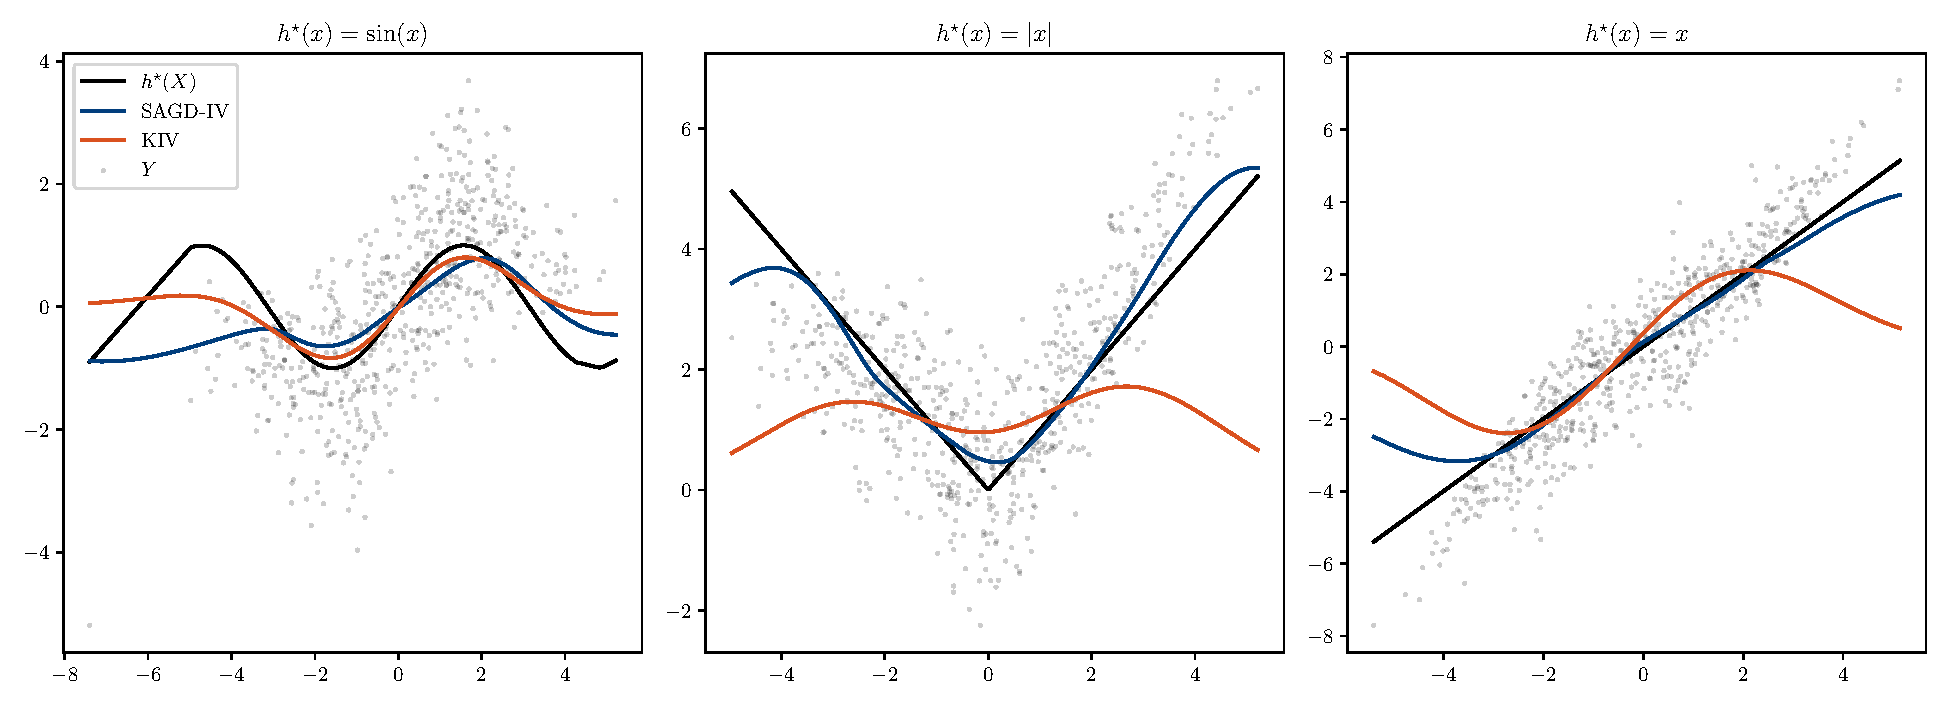
\includegraphics[width=\textwidth]{sagdiv_kiv_comparison.pdf}
            \end{center}
            \caption{Benchmark against Kernel Instrumental Variable (KIV) \cite{singh2019}}
        \end{figure}
    \end{frame}

    \begin{frame}{Future Work}
        \begin{itemize}
            \item<1-> Robust benchmarks against other recent methods;
            \item<1-> Application to discrete outcome models: $ Y = \ind \left\{ \hstar ( X ) + \varepsilon > 0 \right\} $.
        \end{itemize}
    \end{frame}

    \begin{frame}
        \frametitle{References}
        \nocite{*}
        \printbibliography
    \end{frame}

    \begin{frame}
        \centering Thank You!
    \end{frame}

\end{document}
